% don't remove the folling lines, and edit the defintion of \main if needed
\documentclass[../report.tex]{subfiles}
\providecommand{\main}{..}
\IfEq{\jobname}{\currfilebase}{\AtEndDocument{\biblio}}{}
% until here

\begin{document}

\section{Global view of Higgs couplings at the HL/HE-LHC}
\label{sec8}
\begin{center}
\bigskip\vspace{1cm}
{Christopher W. Murphy}
\centerline{{\it Department of Physics, Brookhaven National Laboratory, Upton, New York, 11973, USA}}
\end{center}

\subsection{Introduction}
\label{sec8:intro}
To date there are no conclusive signals of physics beyond the Standard Model (SM) at the Large Hadron Collider (LHC).
This suggests there is a separation of scales between the SM, characterized by $v \approx 246$~GeV, and whatever may lie beyond it at some higher energy, $\Lambda$.
Effective Field Theory (EFT) techniques are ubiquitous in physics, and are most useful when there is a separation of scales in the problem.
Therefore it is not surprising that the Standard Model Effective Field Theory (SMEFT) has become one of the most powerful tools to analyze LHC results given its (near) model-independence, systematic improvability, and ability to simultaneously describe multiple datasets.
Taking a global view of constraints on the Wilson coefficients of the SMEFT is of critical importance not only because these parameters often contribute to multiple datasets, but also because the LHC currently competes in precision with previous generation precision experiments.
Given proposals for future runs of the LHC, High-Luminosity (HL) and High-Energy (HE), it is imperative to understand how the global picture of bounds on Wilson coefficients will change as the HL- and/or HE-LHC become the singularly dominant machine(s) in particle physics.
To do so this Section uses the framework of Ref.~\cite{Ellis:2018gqa}, and its predecessors~\cite{Ellis:2014dva, Ellis:2014jta, Murphy:2017omb}, to project bounds on Wilson coefficients in the SMEFT for the HL and HE runs of the LHC.

\subsection{Standard Model Effective Field Theory}
We focus on dimension-6 operators, and work to linear order in the Warsaw basis~\cite{Grzadkowski:2010es} yielding a consistent EFT expansion to order $O(\Lambda^{-2})$. 
We choose $\alpha$, $G_F$, and $M_Z$ as the input parameters for our computations.
There are 2499 baryon number preserving dimension-6 Wilson coefficients in the SMEFT~\cite{Alonso:2013hga}.
Here we assume a $U(3)^5$ flavor symmetry, one power for each of the five SM fermions fields, under which the Yukawa matrices, $y_{d, e, u}$, are promoted to spurions transforming as bi-triplets.
This reduces the number of (real) coefficients to 76.
However only 20 of those parameters are relevant for the diboson, electroweak precision, and Higgs observables we consider here.

In the Warsaw basis, the 11 operators that span the set of diboson measurements and electroweak precision observables, whether through direct contributions or shifts in input parameters, can be written as  
%
{\small
\begin{align}
\label{eq8:L11}
\mathcal{L}_\text{SMEFT}^\text{Warsaw} &\supset \frac{\bar{C}_{Hl}^{(3)}}{v^2} (H^\dag i\overleftrightarrow{D}^I_\mu H)(\bar l \tau^I \gamma^\mu l) + \frac{\bar{C}_{Hl}^{(1)}}{v^2}(H^\dag i\overleftrightarrow{D}_\mu H)(\bar l \gamma^\mu l) +\frac{\bar{C}_{ll}}{v^2}(\bar l \gamma_\mu l)(\bar l \gamma^\mu l) \nonumber \\
&+ \frac{\bar{C}_{HD}}{v^2}\left|H^\dag D_\mu H\right|^2 + \frac{\bar{C}_{HWB}}{v^2} H^\dag \tau^I H\, W^I_{\mu\nu} B^{\mu\nu}  \nonumber  \\ 
&+ \frac{\bar{C}_{He}}{v^2} (H^\dag i\overleftrightarrow{D}_\mu H)(\bar e \gamma^\mu e) \nonumber + \frac{\bar{C}_{Hu}}{v^2} (H^\dag i\overleftrightarrow{D}_\mu H)(\bar u \gamma^\mu u) + \frac{\bar{C}_{Hd}}{v^2} (H^\dag i\overleftrightarrow{D}_\mu H)(\bar d \gamma^\mu d) \nonumber \\
&+ \frac{\bar{C}_{Hq}^{(3)}}{v^2} (H^\dag i\overleftrightarrow{D}^I_\mu H)(\bar q \tau^I \gamma^\mu q) + \frac{\bar{C}_{Hq}^{(1)}}{v^2} (H^\dag i\overleftrightarrow{D}_\mu H)(\bar q \gamma^\mu q) + \frac{\bar{C}_{W}}{v^2} \epsilon^{IJK} W_\mu^{I\nu} W_\nu^{J\rho} W_\rho^{K\mu} \, ,
\end{align}
}
%
where Hermitian conjugate operators are implicit.
The flavor indices are trivial, except for the four-lepton operator, $C_{ll} = C_{\substack{ll \\ e\mu\mu e}} = C_{\substack{ll \\ \mu ee\mu}}$~\cite{Cirigliano:2009wk}, and are also left implicit.
Additionally in Eq.~\eqref{eq8:L11} we define
%
\begin{equation}
\bar{C} \equiv \frac{v^2}{\Lambda^2}C \, .
\end{equation}
%
There are an additional nine operators that affect Higgs measurements, 
%
{\small
\begin{align}
\label{eq8:L9}
\mathcal{L}_\text{SMEFT}^\text{Warsaw} &\supset  \frac{\bar{C}_{eH}}{v^2} y_e (H^\dag H)(\bar l e H) + \frac{\bar{C}_{dH}}{v^2} y_d (H^\dag H)(\bar q d H) + \frac{\bar{C}_{uH}}{v^2} y_u (H^\dag H)(\bar q u \widetilde H) \nonumber \\
&+ \frac{\bar{C}_{G}}{v^2} f^{ABC} G_\mu^{A\nu} G_\nu^{B\rho} G_\rho^{C\mu}  + \frac{\bar{C}_{H\Box}}{v^2} (H^\dag H)\Box(H^\dag H) + \frac{\bar{C}_{uG}}{v^2} y_u (\bar q \sigma^{\mu\nu} T^A u) \widetilde H \, G_{\mu\nu}^A   \nonumber \\
&+ \frac{\bar{C}_{HW}}{v^2} H^\dag H\, W^I_{\mu\nu} W^{I\mu\nu} + \frac{\bar{C}_{HB}}{v^2}H^\dag H\, B_{\mu\nu} B^{\mu\nu} + \frac{\bar{C}_{HG}}{v^2} H^\dag H\, G^A_{\mu\nu} G^{A\mu\nu} \, .
\end{align}}
The explicit appearance of the Yukawa matrices in Eq.~\eqref{eq8:L9} is necessary to formally preserve the $U(3)^5$ flavor symmetry.
A tenth operator, $\mathcal{O}_H = \left(H^{\dagger} H\right)^3$ operator, is not listed here.
The Wilson coefficient for this operator, $C_H$, can be measured in double-Higgs production, see Section 3 of this report.

Strictly speaking more than nine operators affect Higgs measurements.
All of the operators in Eq.~\eqref{eq8:L11} except $\mathcal{O}_W$ affect Higgs measurements at leading order.
Furthermore Higgs production in association with a top-quark pair probes additional coefficients in the SMEFT~\cite{AguilarSaavedra:2018nen, Ellis:2018gqa} that do not appear in our other observables.
(See also Section 4.1 of this report.)
The only one we explicitly consider is $C_{uG}$, which makes the largest contribution to $t \bar{t} h$ production~\cite{Ellis:2018gqa}. 
An alternative possibility would be to include all the operators by regularizing the fit as in Ref.~\cite{Murphy:2017omb}.
\subsection{Fit Setup and Current Results}
\label{sec8:fit}
We use the predictions for electroweak precision observables and $WW$ scattering at LEP 2 in the Warsaw basis from Refs.~\cite{Berthier:2016tkq, Brivio:2017vri}, whereas predictions for LHC observables are made using $\mathtt{SMEFTsim}$~\cite{Brivio:2017btx}.
The following data are used in our global fit, which are sensitive to 20 directions in the SMEFT parameter space.

\begin{itemize}
\item \textit{pre-LHC data}:  
We use 11 $Z$-pole observables from LEP 1 and 1 from SLC, which are given in Ref.~\cite{ALEPH:2005ab}, as well as the $W$ mass measurement from the Tevatron~\cite{Aaltonen:2013iut}.
In addition we use all the data for the processes $e^+ e^- \to W^+ W^- \to 4f$. 
These measurements were complied in Ref.~\cite{Berthier:2016tkq}, and the original experimental papers are Refs.~\cite{Heister:2004wr, Achard:2004zw, Abbiendi:2007rs, Schael:2013ita}. 
These measurements also probe eleven directions in the SMEFT, which can be mapped to the operators in Eq.~\eqref{eq8:L11}.

\item \textit{LHC Run 1 data}: 
We use all the 20 signal strengths from Table 8 of Ref.~\cite{Khachatryan:2016vau}.
A signal strength is defined as the ratio of the measured cross section to its SM prediction. 
We also use the ATLAS and CMS combination for the $h \to \mu^+ \mu^-$ signal strength~\cite{Khachatryan:2016vau}, and the ATLAS $h \to Z \gamma$ signal strength~\cite{Aad:2015gba}. 
Furthermore, we include the $W$ mass measurements from ATLAS~\cite{Aaboud:2017svj}.

\item \textit{LHC Run 2 data}: 
We use 25 measurements from CMS~\cite{Sirunyan:2017dgc, Sirunyan:2017elk, Sirunyan:2018mvw, Sirunyan:2018shy, CMS-PAS-HIG-16-042, Sirunyan:2018ouh, Sirunyan:2017exp, Sirunyan:2017khh}, and 23 measurements from ATLAS~\cite{Aaboud:2017ojs, Aaboud:2017xsd, Aaboud:2017rss, Aaboud:2017jvq, ATLAS-CONF-2018-004, ATLAS-CONF-2017-047, ATLAS-CONF-2016-112}, including experimental correlations whenever possible. 
In addition we include one measurement of the differential cross section for $p p \to W^+ W^- \to e^{\pm} \nu \mu^{\mp} \nu$, which requires $p_T > 120$~GeV for the leading lepton, by ATLAS at 13~TeV~\cite{Aaboud:2017qkn}.
\end{itemize}

We first present a simplified case where only the operators $C_{HWB}$ and $C_{HD}$ in the Warsaw basis are non-zero.
In this particular case these coefficients are equivalent to the oblique parameters $\Delta S$ and $\Delta T$~\cite{Grinstein:1991cd}
\begin{equation}
\frac{v^2}{\Lambda^2} C_{HWB} = \frac{g_1 g_2}{16 \pi} \Delta S, \quad \frac{v^2}{\Lambda^2} C_{HD} = - \frac{g_1 g_2}{2 \pi \left(g_1 + g_2\right)} \Delta T \, ,
\end{equation}
Figure~\ref{fig8:SandT} shows the preferred parameter space for 
$C_{HWB}$ and $C_{HD}$ for three different selections of the data sets included in the fit.
The blue ellipses are obtained using just pre-LHC measurements in the fit, 
whereas the orange ellipses use only the LHC Run-1 and -2 results.
Finally, the green ellipses are obtained using all the data described in the list above.
The regions shaded in darker and lighter colors are allowed at 1 and 2$\sigma$, respectively. 
%%%%%%%
\begin{figure}[t!]
  \centering
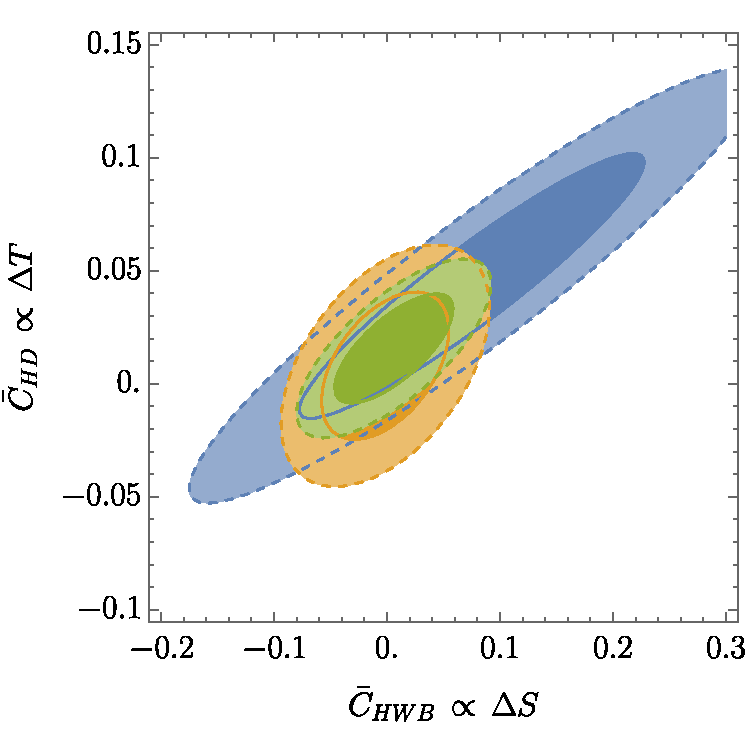
\includegraphics[width=0.6\textwidth]{\main/section8/plots/ST_LHC.pdf}
 \caption{\it Fits to $C_{HWB}$ and $C_{HD}$ using pre-LHC measurements (blue), using LHC Run-1 and -2 results (orange), and all the data (green). The darker and lighter shaded regions are allowed at 1 and 2$\sigma$, respectively. When these are the only two non-zero coefficients in the Warsaw basis they are equivalent to the $\Delta S$ and $\Delta T$ parameters. }
   \label{fig8:SandT}
\end{figure}
%%%%%%%

Fig.~\ref{fig8:HEPfitvsEMSY} summarizes the sensitivities to the scales of the operators in the Warsaw basis.
Specifically it gives the 95\% CL bounds on the sensitivity in TeV for a Wilson coefficient, obtained from marginalized (yellow) and individual (brown) fits to the 20 dimension-6 operators entering in electroweak precision tests, diboson and Higgs measurements at LEP, SLC, Tevatron, and LHC Run-1 and -2.
The yellow and brown bars correspond to the red and green bars of Figure 8 of Ref.~\cite{Ellis:2018gqa}, respectively.
Shown in blue are the analogous results of the individual fits of the HEPfit Collaboration~\cite{Ciuchini:2013pca, deBlas:2016ojx}, see also~\cite{luca:talk, otto:talk}.
For a recent fit in another basis see Ref.~\cite{Alves:2018nof}.
For a recent fit in the Nonlinear Effective Theory see instead Ref.~\cite{deBlas:2018tjm}.
%%%%%%%
\begin{figure}
  \centering
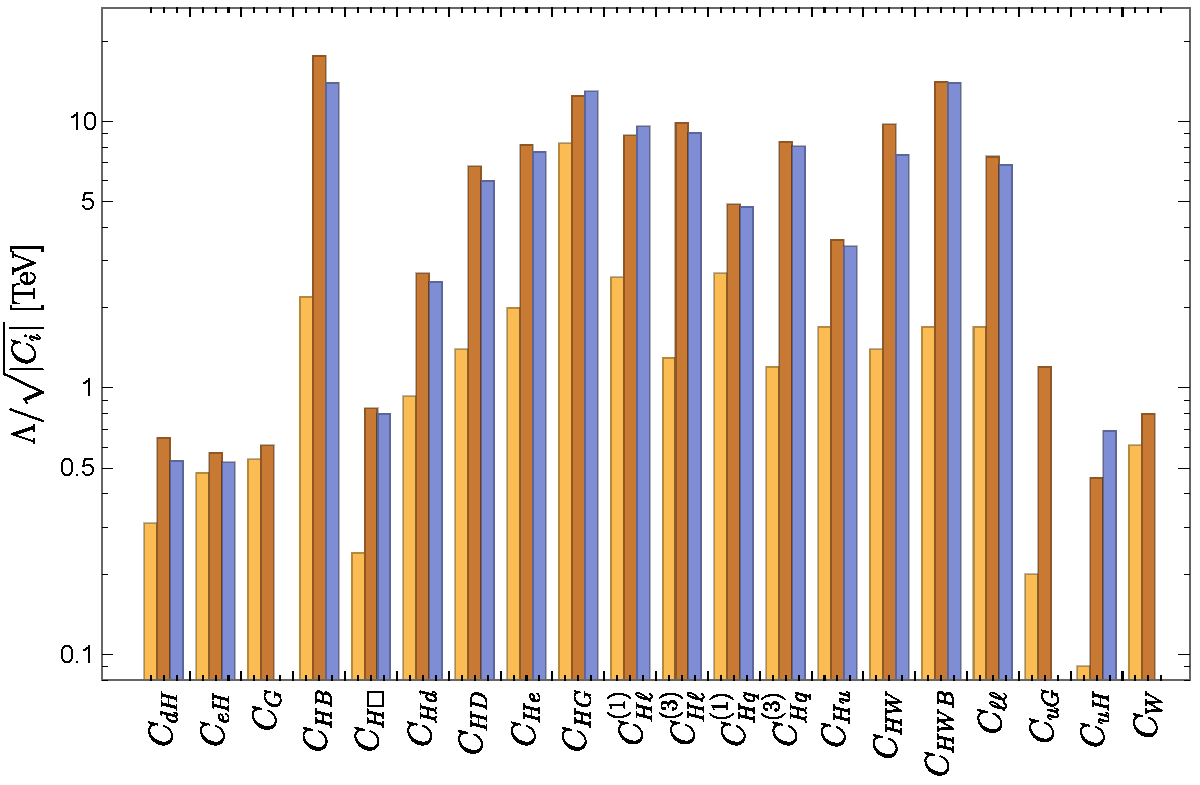
\includegraphics[width=0.8\textwidth]{\main/section8/plots/barcomp.pdf}
 \caption{\it Current constraints on dimension-6 operators. The yellow and brown bars are the marginalized and individual limits from Ref.~\cite{Ellis:2018gqa}, respectively. Shown in blue are the analogous results of the HEPfit Collaboration~\cite{Ciuchini:2013pca, deBlas:2016ojx} for the case where only one operator is switched on at a time.}
   \label{fig8:HEPfitvsEMSY}
\end{figure} 

\subsection{Future Projections}
We project how the bounds on the Wilson coefficients of the SMEFT will change at HL- and HE-LHC using the framework of Ref.~\cite{Ellis:2018gqa}.
Our projection strategy is as follows.
We leave all pre-LHC, and LHC Run-1 measurements unchanged.
For measurements from Run-2 of the LHC we perform two extrapolations as to how the systematic uncertainties will change.
The first, more pessimistic, extrapolation keeps the systematic and theoretical uncertainties fixed to their current values.
This procedure is equivalent to the CMS scenario YR2018 S1~\cite{gilbert:talk}. 
In contrast, the second, more optimistic, extrapolation scales the systematic and theoretical uncertainties as though they were statistical in nature.
This procedure is more optimistic than CMS scenario YR2018 S2 where the theoretical uncertainties are only reduced by a factor of two and there are defined lower limits for the experimental systematic uncertainties~\cite{gilbert:talk}.
In both cases the correlations between experimental measurements are assumed to be unchanged, and the statistical uncertainties are scaled as expected.
In what follows we will refer to the former and the latter scenarios as ``Systematics Unchanged,'' and ``$\sqrt{N}$ Scaling,'' respectively.

The explicit forms of the scaling we use HL- and HE-LHC for the $i^{\text{th}}$ measurement in our dataset are 
\begin{align}
\frac{\delta\mathcal{O}_{\text{HL}, i}}{\delta\mathcal{O}_{\text{today}, i}} = \sqrt{\frac{L_{\text{today}, i}}{L_{\text{HL}}}} , \\
\frac{\delta\mathcal{O}_{\text{HE}, i}}{\delta\mathcal{O}_{\text{today}, i}} = \sqrt{\frac{\sigma_{13, i}}{\sigma_{27, i}} \frac{L_{\text{today}, i}}{L_{\text{HE}}}}  . \nonumber
\end{align}
For the overwhelming majority of the measurements by ATLAS(CMS) $L_{\text{today}, i} = 36.1(35.9)~\text{fb}^{-1}$.
We use the benchmark luminosities $L_{\text{HL}} = 3~\text{ab}^{-1}$. and $L_{\text{HE}} = 15~\text{ab}^{-1}$ for all the measurements in the respective HL and HE extrapolations.
The cross sections $\sigma_{13, i}$ and $\sigma_{27, i}$ refer to the SM cross section in the signal region for a given measurement at 13 and 27 TeV, respectively.

We stress that both our projection scenarios are pessimistic in the sense that they do not take into account the additional channels~\cite{gilbert:talk} and fining binning~\cite{deFlorian:2016spz, Hays:2290628, ATLAS-CONF-2017-047} that will become available as more data are collected.
Furthermore our projections under-utilize LHC diboson scattering measurements, see Sections 4.3 and 4.4 of this report. 

The results of our projections are shown in Figures~\ref{fig8:comp12},~\ref{fig8:comp34},~\ref{fig8:comp56}, and~\ref{fig8:comp78}.
In all four figures the upper panel is a projected fit including all operators simultaneously, whereas the lower panel are projected fits switching each operator on individually.
We display the best-fit values and 95\% CL ranges.
The color coding is consistent throughout the four figures: current bounds (blue), HL-LHC with Systematics Unchanged (orange), HL-LHC with $\sqrt{N}$ Scaling (green), HE-LHC with Systematics Unchanged (red), and HE-LHC with $\sqrt{N}$ Scaling (purple).
The current bounds are displayed in all four figures.
Fig.~\ref{fig8:comp12} shows projections for HL-LHC.
Fig.~\ref{fig8:comp34} shows projections for HE-LHC.
Fig.~\ref{fig8:comp56} shows projections with Systematics Unchanged.
Fig.~\ref{fig8:comp78} shows projections with $\sqrt{N}$ Scaling.
Although Figs.~\ref{fig8:comp12} and~\ref{fig8:comp34} contain all the information from our projections, Figs.~\ref{fig8:comp56} and~\ref{fig8:comp78} are included to make comparisons between different scenarios easier, and vice versa.

In the individual fits there is a large spread in the improvement on the bounds on the Wilson coefficients.
In this scenario some bounds, including those on $C_{dH}$ and $C_{eH}$, improve by an order of magnitude or more, while other bounds, such as those on $C_{He}$ and $C_{H\ell}^{(1)}$, are still dominated by pre-LHC measurements in this particular scenario.
Conversely, when fitting to all operators simultaneously, the general trend is that there is some improvement on the bounds of all of the Wilson coefficients.
Under the $\sqrt{N}$ Scaling scenario HE-LHC clearly outperforms HL-LHC in terms of sensitivity to Wilson coefficients, or equivalently on how large of a cutoff scale $\Lambda$ can be probed.
On the other hand, under the Systematic Unchanged scenario the HL- and HE-LHC perform approximately equally as well as each other in terms of their sensitivity to Wilson coefficients.

%%%%%%%
\begin{figure}
  \centering
  \subfloat{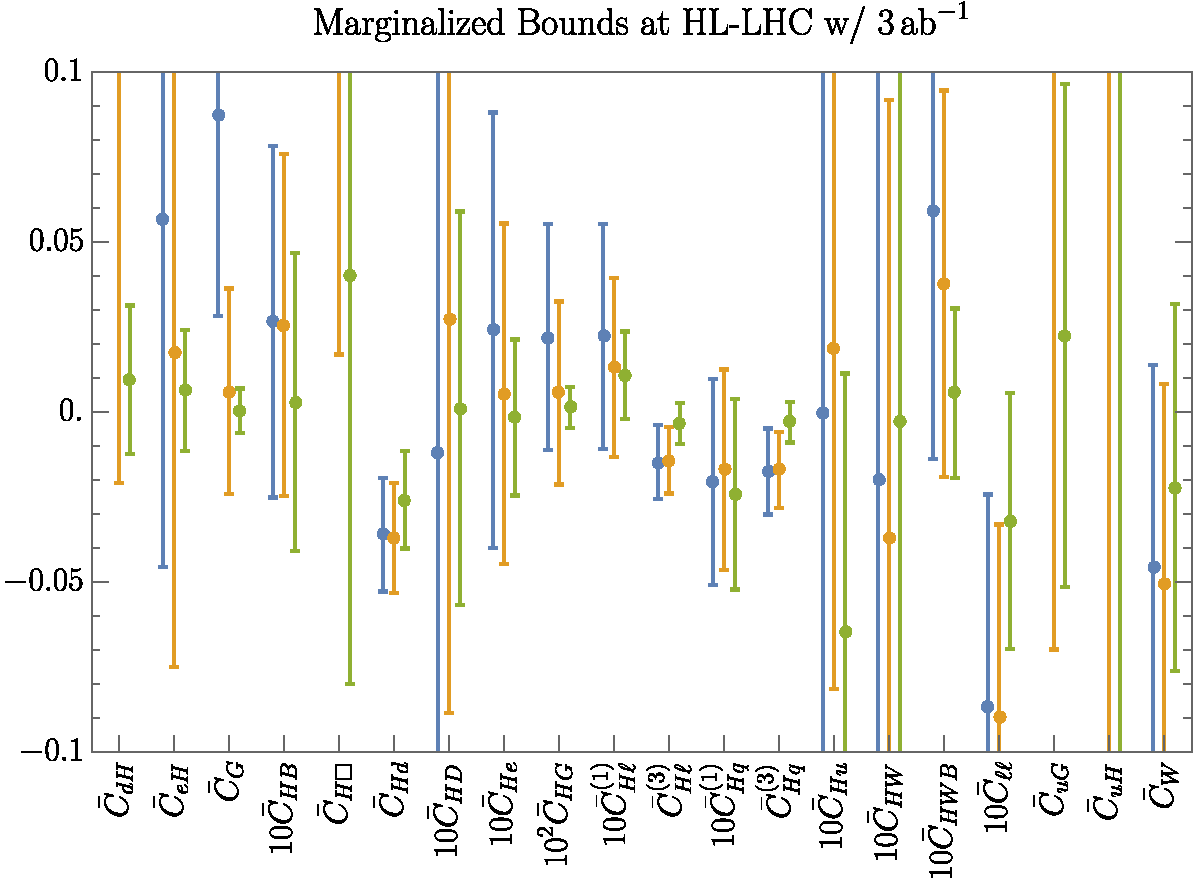
\includegraphics[width=0.85\textwidth]{\main/section8/plots/globalfit_projection1.pdf}}  \\
  \subfloat{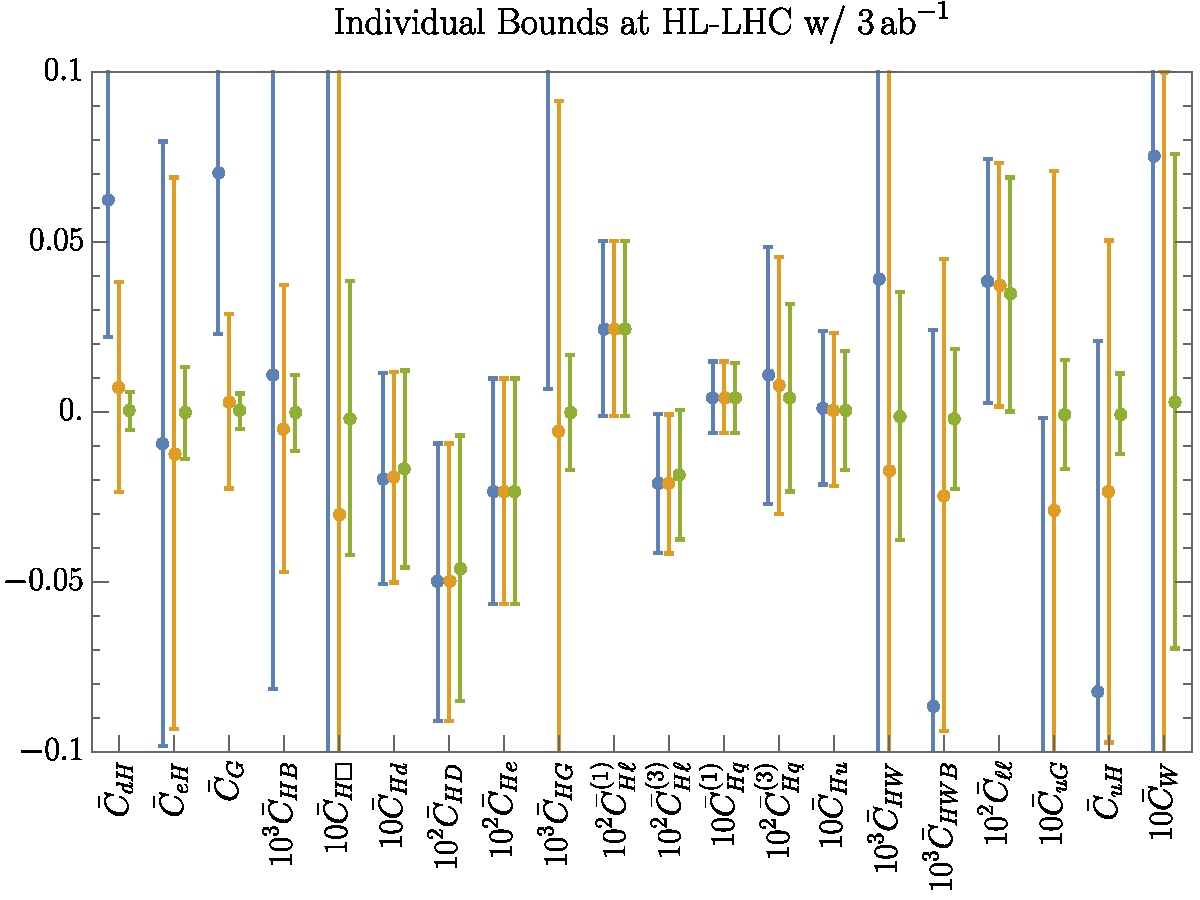
\includegraphics[width=0.85\textwidth]{\main/section8/plots/globalfit_projection2.pdf}}
 \caption{\it Current bounds (blue), and projections for HL-LHC with Systematics Unchanged (orange) and $\sqrt{N}$ Scaling (green) including all operators simultaneously (upper panel) and switching each operator on individually (lower panel). We display the best-fit values and 95\% CL ranges.}
   \label{fig8:comp12}
\end{figure} 

%%%%%%%
\begin{figure}
  \centering
  \subfloat{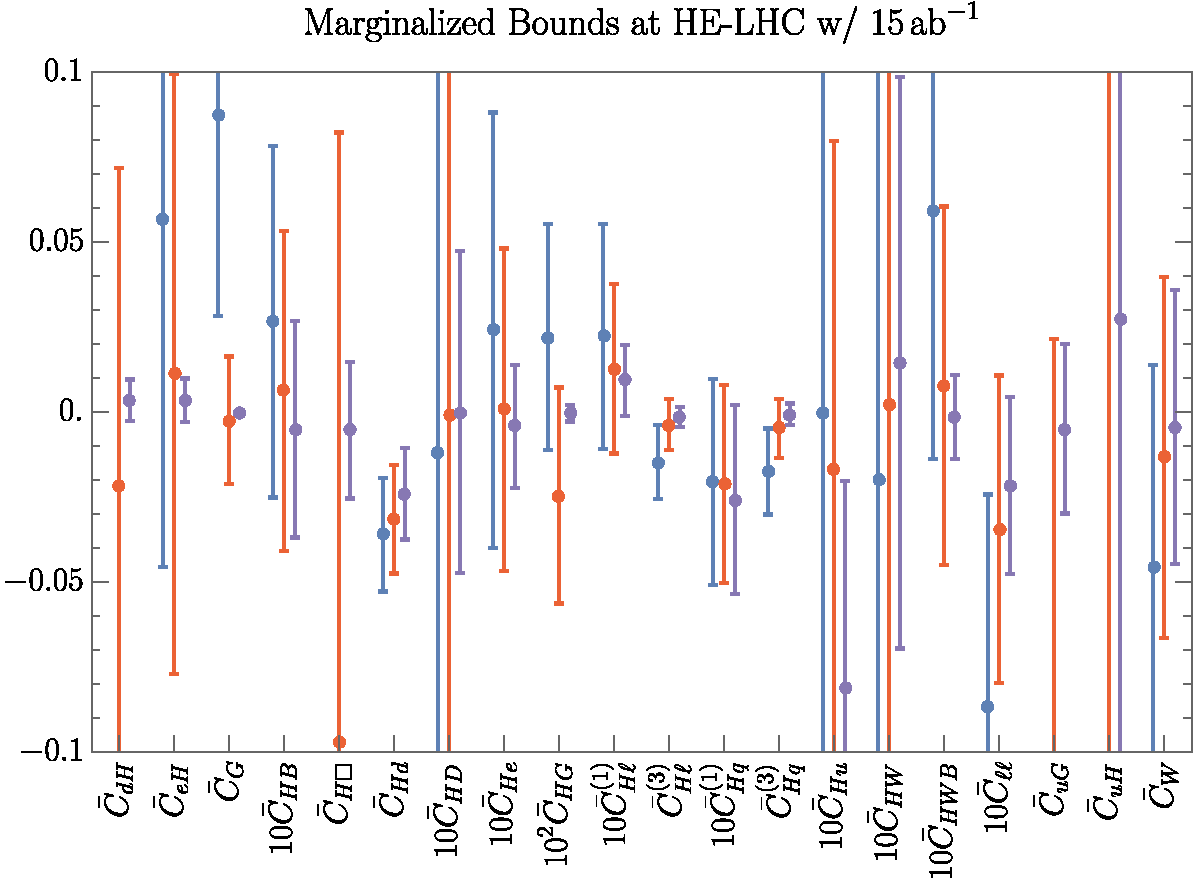
\includegraphics[width=0.85\textwidth]{\main/section8/plots/globalfit_projection3.pdf}}  \\
  \subfloat{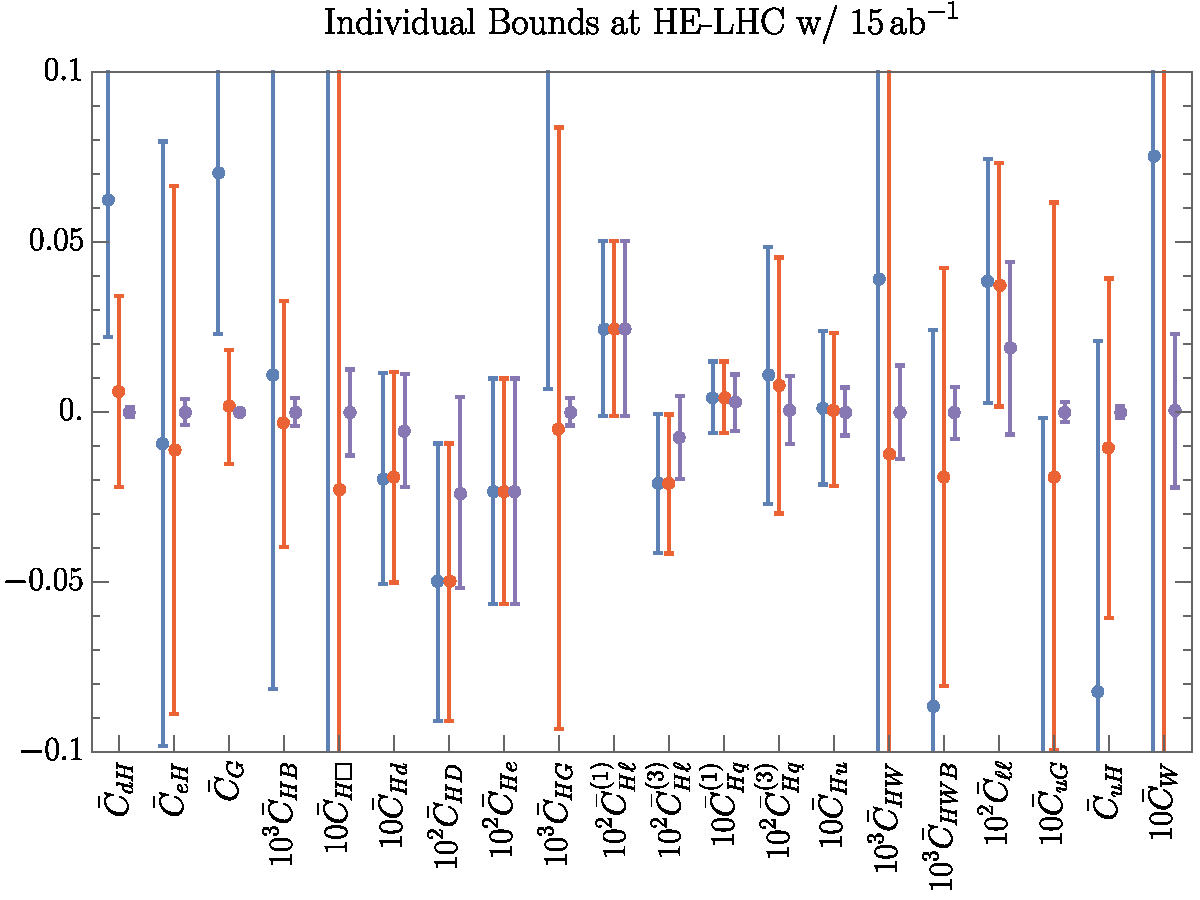
\includegraphics[width=0.85\textwidth]{\main/section8/plots/globalfit_projection4.pdf}}
 \caption{\it Current bounds (blue), and projections for HE-LHC with Systematics Unchanged (red) and $\sqrt{N}$ Scaling (purple) including all operators simultaneously (upper panel) and switching each operator on individually (lower panel). We display the best-fit values and 95\% CL ranges.}
   \label{fig8:comp34}
\end{figure} 

%%%%%%%
\begin{figure}
  \centering
  \subfloat{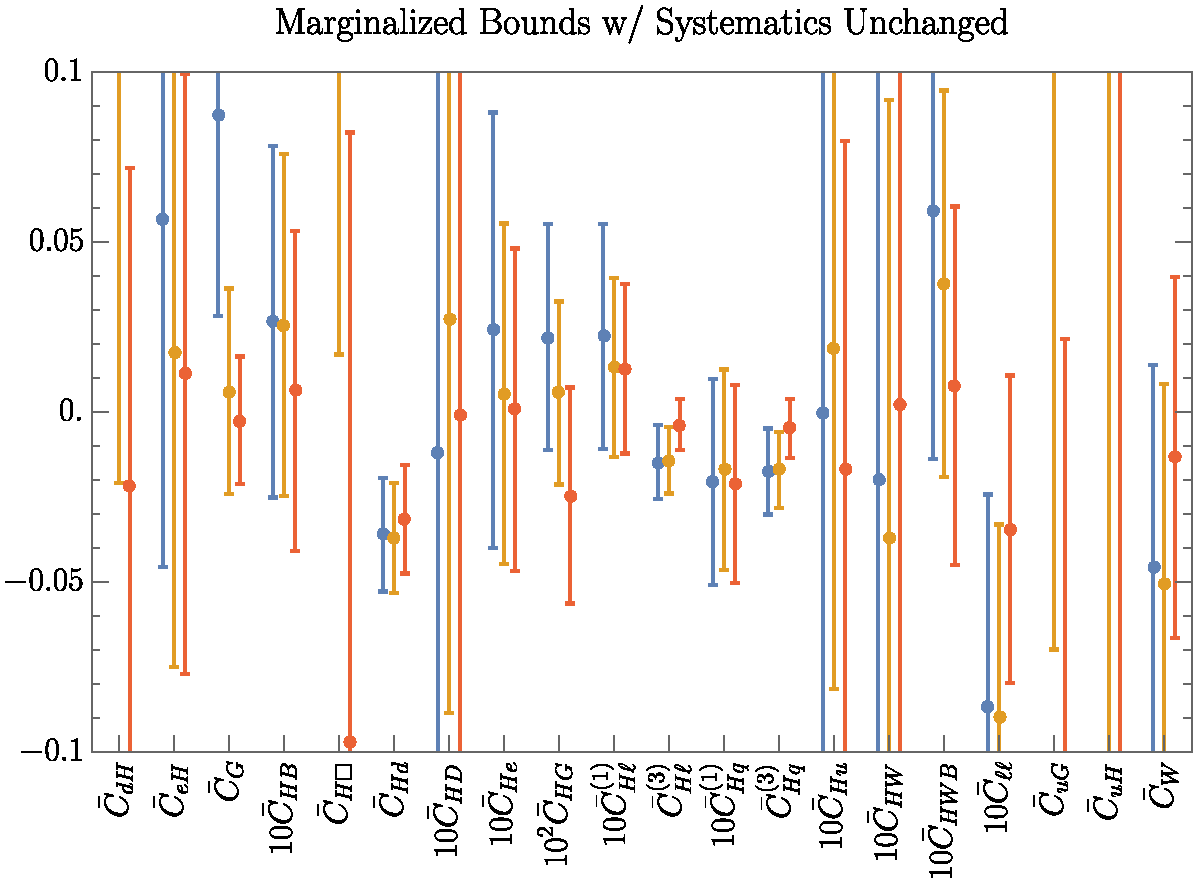
\includegraphics[width=0.85\textwidth]{\main/section8/plots/globalfit_projection5.pdf}}  \\
  \subfloat{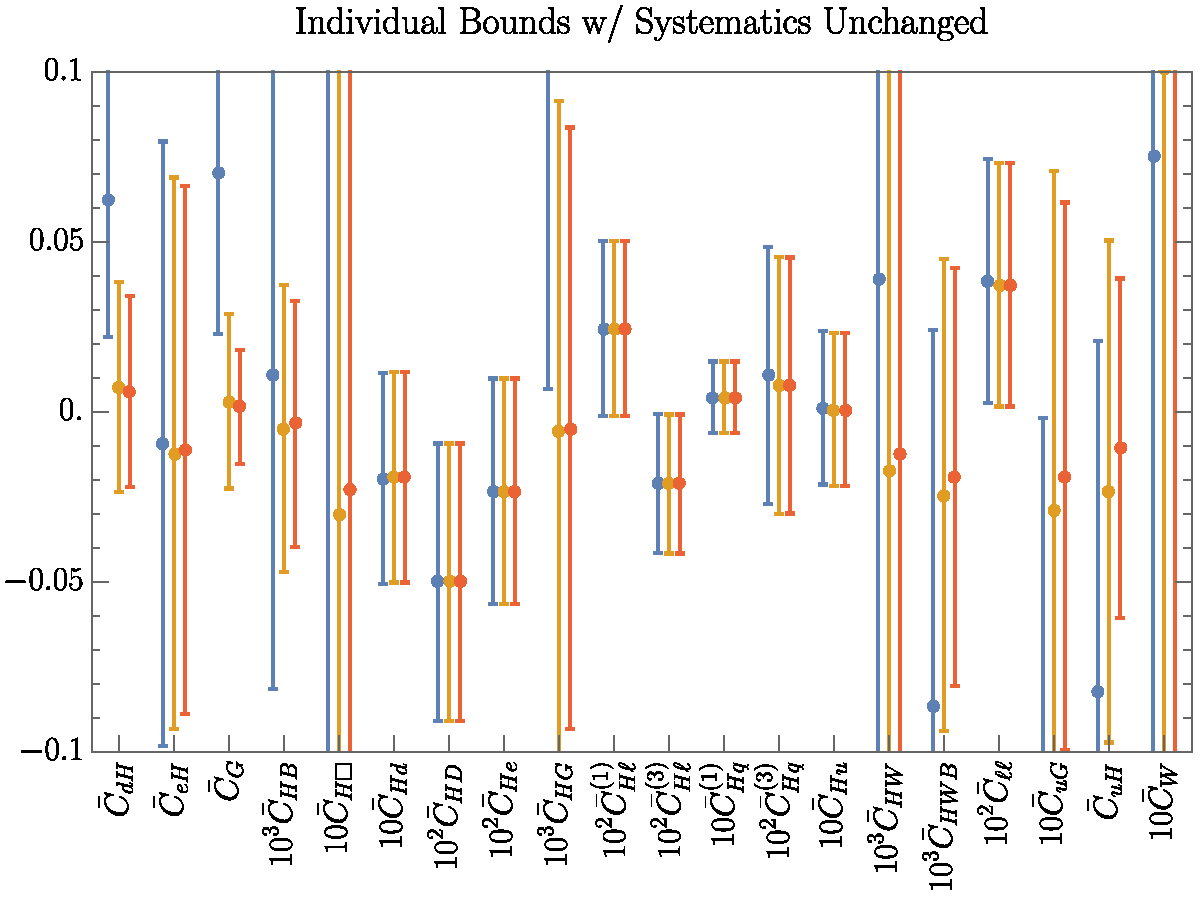
\includegraphics[width=0.85\textwidth]{\main/section8/plots/globalfit_projection6.pdf}}
 \caption{\it Current bounds (blue), and projections with Systematics Unchanged for HL-LHC (orange) and HE-LHC (red) including all operators simultaneously (upper panel) and switching each operator on individually (lower panel). We display the best-fit values and 95\% CL ranges.}
   \label{fig8:comp56}
\end{figure} 

%%%%%%%
\begin{figure}
  \centering
  \subfloat{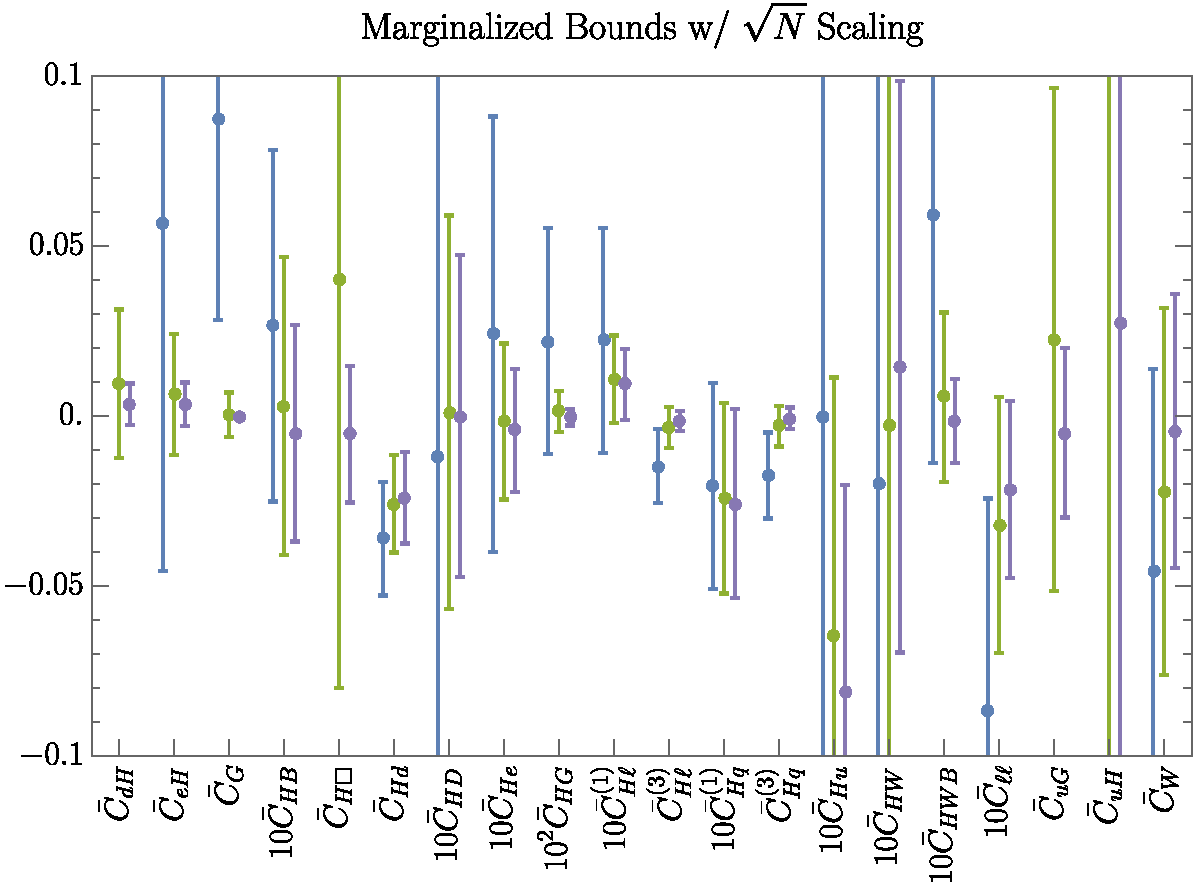
\includegraphics[width=0.85\textwidth]{\main/section8/plots/globalfit_projection7.pdf}}  \\
  \subfloat{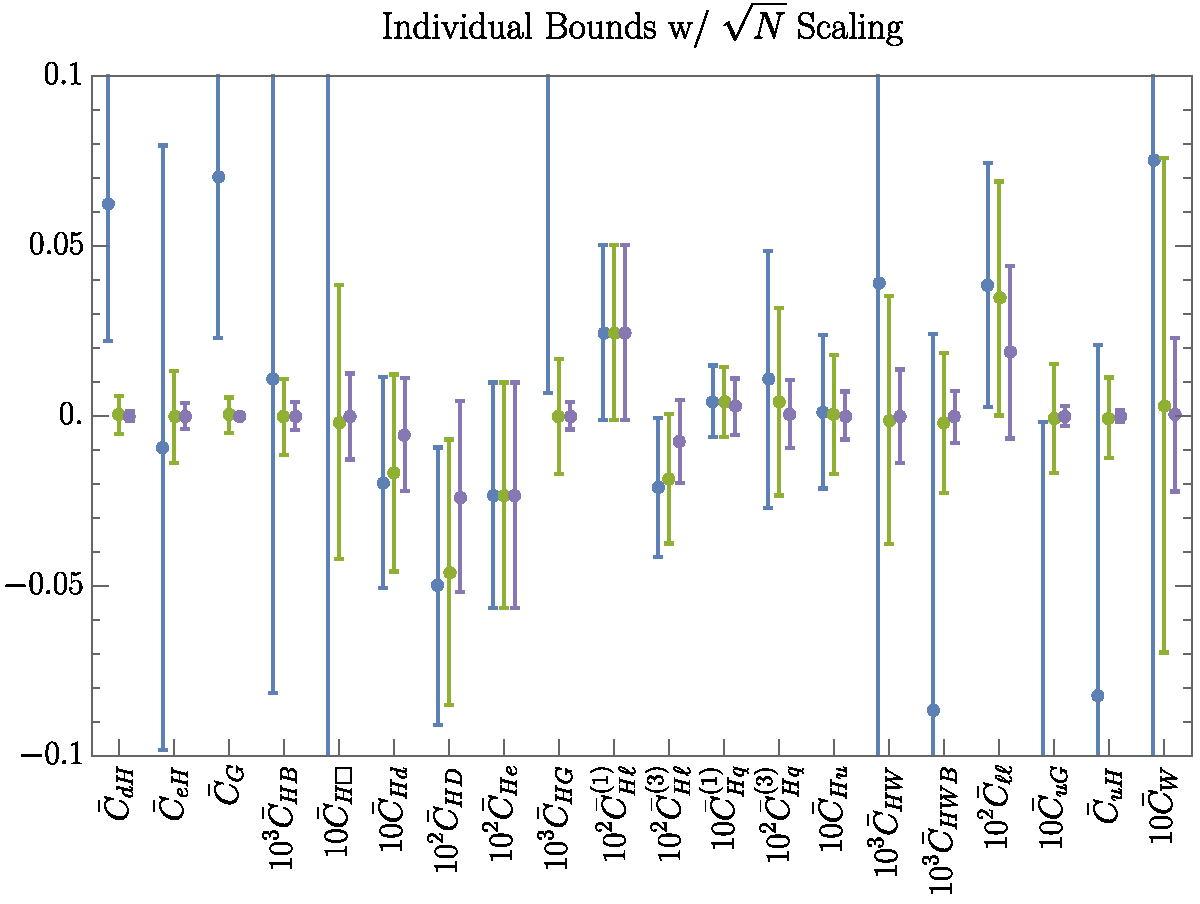
\includegraphics[width=0.85\textwidth]{\main/section8/plots/globalfit_projection8.pdf}}
 \caption{\it Current bounds (blue), and projections with $\sqrt{N}$ scaling for HL-LHC (green) and HE-LHC (purple) including all operators simultaneously (upper panel) and switching each operator on individually (lower panel). We display the best-fit values and 95\% CL ranges.}
   \label{fig8:comp78}
\end{figure}

Acknowledgments: 
%%%%%%%%%%%%%%%%%%%%%%%%%
CM thanks John Ellis, Ver\'{o}nica Sanz, and Tevong You for collaborations on Ref.~\cite{Ellis:2018gqa}.
The work of CM was supported by the United States Department of Energy under Grant Contract DE-SC0012704.

\end{document}
